\PassOptionsToPackage{unicode=true}{hyperref} % options for packages loaded elsewhere
\PassOptionsToPackage{hyphens}{url}
%
\documentclass[ignorenonframetext,]{beamer}
\usepackage{pgfpages}
\setbeamertemplate{caption}[numbered]
\setbeamertemplate{caption label separator}{: }
\setbeamercolor{caption name}{fg=normal text.fg}
\beamertemplatenavigationsymbolsempty
% Prevent slide breaks in the middle of a paragraph:
\widowpenalties 1 10000
\raggedbottom
\setbeamertemplate{part page}{
\centering
\begin{beamercolorbox}[sep=16pt,center]{part title}
  \usebeamerfont{part title}\insertpart\par
\end{beamercolorbox}
}
\setbeamertemplate{section page}{
\centering
\begin{beamercolorbox}[sep=12pt,center]{part title}
  \usebeamerfont{section title}\insertsection\par
\end{beamercolorbox}
}
\setbeamertemplate{subsection page}{
\centering
\begin{beamercolorbox}[sep=8pt,center]{part title}
  \usebeamerfont{subsection title}\insertsubsection\par
\end{beamercolorbox}
}
\AtBeginPart{
  \frame{\partpage}
}
\AtBeginSection{
  \ifbibliography
  \else
    \frame{\sectionpage}
  \fi
}
\AtBeginSubsection{
  \frame{\subsectionpage}
}
\usepackage{lmodern}
\usepackage{amssymb,amsmath}
\usepackage{ifxetex,ifluatex}
\usepackage{fixltx2e} % provides \textsubscript
\ifnum 0\ifxetex 1\fi\ifluatex 1\fi=0 % if pdftex
  \usepackage[T1]{fontenc}
  \usepackage[utf8]{inputenc}
  \usepackage{textcomp} % provides euro and other symbols
\else % if luatex or xelatex
  \usepackage{unicode-math}
  \defaultfontfeatures{Ligatures=TeX,Scale=MatchLowercase}
\fi
\usetheme[]{AnnArbor}
\usecolortheme{beaver}
\usefonttheme{structurebold}
% use upquote if available, for straight quotes in verbatim environments
\IfFileExists{upquote.sty}{\usepackage{upquote}}{}
% use microtype if available
\IfFileExists{microtype.sty}{%
\usepackage[]{microtype}
\UseMicrotypeSet[protrusion]{basicmath} % disable protrusion for tt fonts
}{}
\IfFileExists{parskip.sty}{%
\usepackage{parskip}
}{% else
\setlength{\parindent}{0pt}
\setlength{\parskip}{6pt plus 2pt minus 1pt}
}
\usepackage{hyperref}
\hypersetup{
            pdftitle={Causalité},
            pdfauthor={Visseho Adjiwanou, PhD.},
            pdfborder={0 0 0},
            breaklinks=true}
\urlstyle{same}  % don't use monospace font for urls
\newif\ifbibliography
\usepackage{color}
\usepackage{fancyvrb}
\newcommand{\VerbBar}{|}
\newcommand{\VERB}{\Verb[commandchars=\\\{\}]}
\DefineVerbatimEnvironment{Highlighting}{Verbatim}{commandchars=\\\{\}}
% Add ',fontsize=\small' for more characters per line
\usepackage{framed}
\definecolor{shadecolor}{RGB}{248,248,248}
\newenvironment{Shaded}{\begin{snugshade}}{\end{snugshade}}
\newcommand{\AlertTok}[1]{\textcolor[rgb]{0.94,0.16,0.16}{#1}}
\newcommand{\AnnotationTok}[1]{\textcolor[rgb]{0.56,0.35,0.01}{\textbf{\textit{#1}}}}
\newcommand{\AttributeTok}[1]{\textcolor[rgb]{0.77,0.63,0.00}{#1}}
\newcommand{\BaseNTok}[1]{\textcolor[rgb]{0.00,0.00,0.81}{#1}}
\newcommand{\BuiltInTok}[1]{#1}
\newcommand{\CharTok}[1]{\textcolor[rgb]{0.31,0.60,0.02}{#1}}
\newcommand{\CommentTok}[1]{\textcolor[rgb]{0.56,0.35,0.01}{\textit{#1}}}
\newcommand{\CommentVarTok}[1]{\textcolor[rgb]{0.56,0.35,0.01}{\textbf{\textit{#1}}}}
\newcommand{\ConstantTok}[1]{\textcolor[rgb]{0.00,0.00,0.00}{#1}}
\newcommand{\ControlFlowTok}[1]{\textcolor[rgb]{0.13,0.29,0.53}{\textbf{#1}}}
\newcommand{\DataTypeTok}[1]{\textcolor[rgb]{0.13,0.29,0.53}{#1}}
\newcommand{\DecValTok}[1]{\textcolor[rgb]{0.00,0.00,0.81}{#1}}
\newcommand{\DocumentationTok}[1]{\textcolor[rgb]{0.56,0.35,0.01}{\textbf{\textit{#1}}}}
\newcommand{\ErrorTok}[1]{\textcolor[rgb]{0.64,0.00,0.00}{\textbf{#1}}}
\newcommand{\ExtensionTok}[1]{#1}
\newcommand{\FloatTok}[1]{\textcolor[rgb]{0.00,0.00,0.81}{#1}}
\newcommand{\FunctionTok}[1]{\textcolor[rgb]{0.00,0.00,0.00}{#1}}
\newcommand{\ImportTok}[1]{#1}
\newcommand{\InformationTok}[1]{\textcolor[rgb]{0.56,0.35,0.01}{\textbf{\textit{#1}}}}
\newcommand{\KeywordTok}[1]{\textcolor[rgb]{0.13,0.29,0.53}{\textbf{#1}}}
\newcommand{\NormalTok}[1]{#1}
\newcommand{\OperatorTok}[1]{\textcolor[rgb]{0.81,0.36,0.00}{\textbf{#1}}}
\newcommand{\OtherTok}[1]{\textcolor[rgb]{0.56,0.35,0.01}{#1}}
\newcommand{\PreprocessorTok}[1]{\textcolor[rgb]{0.56,0.35,0.01}{\textit{#1}}}
\newcommand{\RegionMarkerTok}[1]{#1}
\newcommand{\SpecialCharTok}[1]{\textcolor[rgb]{0.00,0.00,0.00}{#1}}
\newcommand{\SpecialStringTok}[1]{\textcolor[rgb]{0.31,0.60,0.02}{#1}}
\newcommand{\StringTok}[1]{\textcolor[rgb]{0.31,0.60,0.02}{#1}}
\newcommand{\VariableTok}[1]{\textcolor[rgb]{0.00,0.00,0.00}{#1}}
\newcommand{\VerbatimStringTok}[1]{\textcolor[rgb]{0.31,0.60,0.02}{#1}}
\newcommand{\WarningTok}[1]{\textcolor[rgb]{0.56,0.35,0.01}{\textbf{\textit{#1}}}}
\usepackage{longtable,booktabs}
\usepackage{caption}
% These lines are needed to make table captions work with longtable:
\makeatletter
\def\fnum@table{\tablename~\thetable}
\makeatother
\usepackage{graphicx,grffile}
\makeatletter
\def\maxwidth{\ifdim\Gin@nat@width>\linewidth\linewidth\else\Gin@nat@width\fi}
\def\maxheight{\ifdim\Gin@nat@height>\textheight\textheight\else\Gin@nat@height\fi}
\makeatother
% Scale images if necessary, so that they will not overflow the page
% margins by default, and it is still possible to overwrite the defaults
% using explicit options in \includegraphics[width, height, ...]{}
\setkeys{Gin}{width=\maxwidth,height=\maxheight,keepaspectratio}
\setlength{\emergencystretch}{3em}  % prevent overfull lines
\providecommand{\tightlist}{%
  \setlength{\itemsep}{0pt}\setlength{\parskip}{0pt}}
\setcounter{secnumdepth}{0}

% set default figure placement to htbp
\makeatletter
\def\fps@figure{htbp}
\makeatother

\usepackage{color}

\title{Causalité}
\author{Visseho Adjiwanou, PhD.}
\providecommand{\institute}[1]{}
\institute{Département de Sociologie - UQAM}
\date{28 Janvier 2019}

\begin{document}
\frame{\titlepage}

\begin{frame}{Plan de présentation}
\protect\hypertarget{plan-de-presentation}{}

\begin{enumerate}
\item
  Questions causales en sciences sociales et terminologie
\item
  Effets causaux et contrefactuel
\item
  Essais contrôlés randomisés (\emph{Randomized controlled trials}) et
  causalité
\item
  Causalité à partir des données observationnelles
\item
  Exercices
\end{enumerate}

\end{frame}

\hypertarget{introduction}{%
\section{Introduction}\label{introduction}}

\begin{frame}{Introduction}
\protect\hypertarget{introduction-1}{}

\begin{itemize}
\tightlist
\item
  Dans ce chapitre, nous considérons la causalité, l'un des concepts les
  plus centraux des sciences sociales quantitatives.
\item
  Une grande partie de la recherche en sciences sociales s'intéresse aux
  effets causaux de diverses politiques et autres facteurs sociétaux.
\item
  Par exemple:

  \begin{itemize}
  \tightlist
  \item
    Est-ce que le vaccin A protège contre la maladie X?
  \item
    Les classes de petite taille augmentent-elles les résultats des
    tests standardisés des élèves?
  \item
    Les soins de santé universels amélioreraient-ils la santé et les
    finances des pauvres?
  \item
    L'éducation réduit-elle le nombre d'enfants?
  \item
    La rémunération des gens sur Wikipedia augmentera-elle leur
    productivité?
  \item
    Est-ce que l'augmentation du salaire minimum réduit l'activité
    économique?
  \end{itemize}
\end{itemize}

\end{frame}

\hypertarget{questions-de-recherche}{%
\section{Questions de recherche}\label{questions-de-recherche}}

\begin{frame}{Questions de recherche}
\protect\hypertarget{questions-de-recherche-1}{}

\begin{itemize}
\tightlist
\item
  Une question de recherche est au cœur d'un projet de recherche, d'une
  étude ou d'une revue de littérature.
\item
  Il concentre l'étude, détermine la méthodologie et guide toutes les
  étapes de la recherche, de l'analyse et de la production de rapports.
\item
  Peut être \textbf{associatif} ou \textbf{causal}
\end{itemize}

\end{frame}

\begin{frame}{Exemple 1}
\protect\hypertarget{exemple-1}{}

\begin{enumerate}
\tightlist
\item
  Le salaire minimum augmente-t-il le taux de chômage?

  \begin{itemize}
  \tightlist
  \item
    Le taux de chômage a augmenté après l'augmentation du salaire
    minimum.
  \item
    Le taux de chômage aurait-il augmenté si l'augmentation du salaire
    minimum n'avait pas eu lieu?
  \end{itemize}
\end{enumerate}

\end{frame}

\begin{frame}{Exemple 2}
\protect\hypertarget{exemple-2}{}

\begin{enumerate}
\setcounter{enumi}{1}
\tightlist
\item
  La race/l'ethnie a-t-elle une incidence sur les perspectives d'emploi?

  \begin{itemize}
  \tightlist
  \item
    Mohamed a postulé pour un emploi mais ne l'a pas obtenu.
  \item
    Mohamed aurait-il trouvé un travail s'il était blanc (avait un nom
    européen)?
  \end{itemize}
\end{enumerate}

\end{frame}

\begin{frame}{Exemple 3}
\protect\hypertarget{exemple-3}{}

\begin{enumerate}
\setcounter{enumi}{2}
\tightlist
\item
  Est-ce que fumer cause une maladie coronarienne?

  \begin{itemize}
  \tightlist
  \item
    Jean, fumeur, a eu une maladie coronarienne.
  \item
    Est-ce que Jean aurait eu la même maladie s'il n'était pas fumeur?
  \end{itemize}
\end{enumerate}

\end{frame}

\begin{frame}{Exemple 4}
\protect\hypertarget{exemple-4}{}

\begin{enumerate}
\setcounter{enumi}{3}
\tightlist
\item
  Quelle est l'importance des questions souverainistes dans la victoire
  de François Legault?

  \begin{itemize}
  \tightlist
  \item
    Au cours de ces élections, la question souverainiste a été laissé de
    côté et François Legault a gagné.
  \item
    François Legault aurait-il gagné les élections si ces questions
    étaient présentes?
  \end{itemize}
\end{enumerate}

\end{frame}

\begin{frame}{Terminologie}
\protect\hypertarget{terminologie}{}

\begin{enumerate}
\tightlist
\item
  \textbf{Réponse ou variable dépendante}, \emph{outcome}
\end{enumerate}

\begin{itemize}
\tightlist
\item
  C'est ce que nous voulons expliquer.
\item
  \emph{Exemples}:

  \begin{itemize}
  \tightlist
  \item
    Taux de chômage
  \item
    Perspective d'emploi
  \item
    Maladie coronarienne
  \item
    Victoire de François Legault
  \end{itemize}
\end{itemize}

\end{frame}

\begin{frame}{Terminologie}
\protect\hypertarget{terminologie-1}{}

\begin{enumerate}
\setcounter{enumi}{1}
\tightlist
\item
  \textbf{Variable indépendante, facteur de risque}
\end{enumerate}

\begin{itemize}
\tightlist
\item
  Tout facteur pouvant influencer la variable de réponse
\item
  Peut être de différents niveaux
\item
  Leur choix dépend de la théorie
\item
  \emph{Exemples}:

  \begin{itemize}
  \tightlist
  \item
    Salaire minimum
  \item
    Ethnie / Race
  \item
    Fumer
  \item
    Questions souverainistes
  \end{itemize}
\end{itemize}

\begin{enumerate}
\setcounter{enumi}{2}
\tightlist
\item
  \textbf{Variables de contrôle}
\end{enumerate}

\end{frame}

\hypertarget{type-de-relation}{%
\section{Type de relation}\label{type-de-relation}}

\begin{frame}{Association}
\protect\hypertarget{association}{}

\begin{itemize}
\tightlist
\item
  On dit que deux variables A et B sont \textbf{associées} quand l'une
  se trouve plus communément en présence de l'autre.
\item
  Se détecte souvent à partir d'un tableau dit de \textbf{contingence}
  ou \textbf{tableau croisé} ou d'un graphique
\item
  Exemple - Existe-il une association entre le degré d'ouverture d'un
  pays et l'attitude face a la violence contre les femmes?
\end{itemize}

Pierotti, Rachel. (2013).
``\href{http://dx.doi.org/10.1177/0003122413480363}{Increasing Rejection
of Intimate Partner Violence: Evidence of Global Cultural Diffusion}.''
\emph{American Sociological Review}, 78: 240-265.

Nous utilisons les données des enquêtes démographiques et de santé
(EDS), qui représentent un ensemble de plus de 300 enquêtes
représentatives à l'échelle nationale, régionale et résidentielle menées
dans des pays en développement du monde entier depuis 1992.

\end{frame}

\begin{frame}[fragile]{Association}
\protect\hypertarget{association-1}{}

\begin{longtable}[]{@{}ll@{}}
\toprule
Name & Description\tabularnewline
\midrule
\endhead
\texttt{beat\_burnfood} & Pourcentage de femmes dans chaque pays
qui\tabularnewline
& pensent qu'un mari a le droit de battre sa femme\tabularnewline
& si elle brûle la nourriture (quantitative)\tabularnewline
\texttt{beat\_burnfood\_cat} & Variable beat\_bunfood en 4 catégories
(qualitative)\tabularnewline
\texttt{no\_media} & Pourcentage de femmes dans chaque pays qui
ont\tabularnewline
& rarement accès un journal, une radio ou une\tabularnewline
& télévision (quantitative)\tabularnewline
\texttt{no\_media\_cat} & Variable no\_media en 3 catégories
(qualitative)\tabularnewline
\texttt{country} & pays\tabularnewline
\bottomrule
\end{longtable}

\end{frame}

\begin{frame}[fragile]{Association}
\protect\hypertarget{association-2}{}

\begin{verbatim}
## [1] "/Users/visseho/OneDrive - UQAM/Cours/SOC2206/Seances/Semaine5_causalite"
\end{verbatim}

\begin{verbatim}
## # A tibble: 6 x 11
##      X1 beat_burnfood beat_goesout sec_school no_media country  year region
##   <dbl>         <dbl>        <dbl>      <dbl>    <dbl> <chr>   <dbl> <chr> 
## 1     1           4.4         18.6       25.2      1.5 Albania  2008 Middl~
## 2     4           4.9         19.9       67.7      8.7 Armenia  2000 Middl~
## 3     5           2.1         10.3       67.6      2.2 Armenia  2005 Middl~
## 4     6           0.3          3.1       46        6.4 Armenia  2010 Middl~
## 5     7          12.1         42.5       74.6      7.4 Azerba~  2006 Middl~
## 6     8          NA           NA         24       41.9 Bangla~  2004 Asia  
## # ... with 3 more variables: beat_burnfood_cat <fct>,
## #   beat_goesout_cat <fct>, no_media_cat <fct>
\end{verbatim}

\end{frame}

\begin{frame}[fragile]{Association}
\protect\hypertarget{association-3}{}

\begin{itemize}
\tightlist
\item
  Résumé de l'information contenue dans la base de donnée
\end{itemize}

\begin{verbatim}
##        X1         beat_burnfood    beat_goesout     sec_school   
##  Min.   :  1.00   Min.   : 0.10   Min.   : 0.30   Min.   : 3.10  
##  1st Qu.: 40.50   1st Qu.: 4.50   1st Qu.:11.85   1st Qu.:10.18  
##  Median : 79.00   Median :11.85   Median :28.10   Median :22.40  
##  Mean   : 80.53   Mean   :15.04   Mean   :28.60   Mean   :24.40  
##  3rd Qu.:119.50   3rd Qu.:22.25   3rd Qu.:42.08   3rd Qu.:34.90  
##  Max.   :160.00   Max.   :64.50   Max.   :82.70   Max.   :74.60  
##                   NA's   :31      NA's   :27      NA's   :3      
##     no_media       country               year         region         
##  Min.   : 0.80   Length:151         Min.   :1999   Length:151        
##  1st Qu.:11.25   Class :character   1st Qu.:2004   Class :character  
##  Median :29.15   Mode  :character   Median :2007   Mode  :character  
##  Mean   :28.40                      Mean   :2007                     
##  3rd Qu.:43.23                      3rd Qu.:2011                     
##  Max.   :86.40                      Max.   :2014                     
##  NA's   :13                                                          
##    beat_burnfood_cat    beat_goesout_cat no_media_cat
##  Très faible:30      Très faible:31      Riche :46   
##  Faible     :30      Faible     :31      Moyen :46   
##  Élevé      :30      Élevé      :31      Pauvre:46   
##  Très élevé :30      Très élevé :31      NA's  :13   
##  NA's       :31      NA's       :27                  
##                                                      
## 
\end{verbatim}

\end{frame}

\begin{frame}{Association}
\protect\hypertarget{association-4}{}

\begin{itemize}
\tightlist
\item
  Association entre deux variables qualitatives
\end{itemize}

\includegraphics{Causalite_Visseho_Adjiwanou_files/figure-beamer/unnamed-chunk-3-1.pdf}

\end{frame}

\begin{frame}{Association}
\protect\hypertarget{association-5}{}

\begin{itemize}
\tightlist
\item
  Représentation graphique (boxplot) dans le cas d'une variable
  qualitative et d'une variable quantitative
\end{itemize}

\includegraphics[width=0.75\linewidth]{Causalite_Visseho_Adjiwanou_files/figure-beamer/unnamed-chunk-4-1}

\end{frame}

\begin{frame}{Association}
\protect\hypertarget{association-6}{}

\begin{itemize}
\tightlist
\item
  Représentation linéaire (scatterplot) et de calcul d'indicateurs
  (corrélation de Pearson): dans le cas de deux variables quantitatives.
\end{itemize}

\includegraphics[width=0.75\linewidth]{Causalite_Visseho_Adjiwanou_files/figure-beamer/unnamed-chunk-5-1}

\end{frame}

\begin{frame}{Association}
\protect\hypertarget{association-7}{}

\includegraphics[width=0.75\linewidth]{Causalite_Visseho_Adjiwanou_files/figure-beamer/unnamed-chunk-6-1}

\end{frame}

\begin{frame}{Relation associative}
\protect\hypertarget{relation-associative}{}

\begin{itemize}
\tightlist
\item
  Une association (linéaire) peut être

  \begin{itemize}
  \tightlist
  \item
    \textbf{positive} si les deux variables vont dans le même sens (une
    augmentation de l'un est associée à une augmentation de l'autre);

    \begin{itemize}
    \tightlist
    \item
      \emph{Exemple} : éducation et revenu, durée de résidence et emploi
    \end{itemize}
  \item
    \textbf{négative} si les deux variables vont dans des sens opposés
    (une augmentation de l'un est associée à une diminution de l'autre);

    \begin{itemize}
    \tightlist
    \item
      \emph{Exemple} : scolarisation et racisme, revenu et obésité,
      niveau de développement d'un pays et niveau de mortalité infantile
    \end{itemize}
  \item
    \textbf{nulle} (Absence d'association).

    \begin{itemize}
    \tightlist
    \item
      \emph{Exemple}:
    \end{itemize}
  \end{itemize}
\end{itemize}

\end{frame}

\begin{frame}{Relation causale}
\protect\hypertarget{relation-causale}{}

\begin{itemize}
\tightlist
\item
  L'association est une \textbf{condition nécessaire} à la causalité
  (Mais elle \textbf{n'est pas suffisante}).
\item
  Toutes les associations ne sont pas causales. L'association peut
  arriver par hasard.
\item
  \textbf{L'analyse statistique à elle seule ne peut constituer une
  preuve d'un lien de causalité}
\item
  Comparaison entre \textbf{\(\color{red}{factuel}\)} et
  \textbf{\(\color{red}{contrefactuel}\)}
\item
  Problème fondamental de l'inférence causale:

  \begin{itemize}
  \tightlist
  \item
    Il faut déduire des résultats contrefactuels
  \item
    Il n'y a pas de causalité sans manipulation: caractéristiques
    immuables
  \end{itemize}
\end{itemize}

\end{frame}

\begin{frame}{Relation causale}
\protect\hypertarget{relation-causale-1}{}

\begin{itemize}
\item
  La clé pour comprendre la causalité est de penser au contrefactuel.
  L'inférence causale est une comparaison entre le factuel (ce qui s'est
  réellement passé) et le contrefactuel (ce qui se serait passé si une
  condition était différente).
\item
  Contrefactuels ne sont pas observés, sauf dans les films.
\item
  \url{https://www.youtube.com/watch?v=BvUbv4iwbDs\&rel=0\&modestbranding=1\&autohide=1\&showinfo=0}
\end{itemize}

\end{frame}

\hypertarget{essais-controles-randomises-experimentation}{%
\section{Essais contrôlés randomisés
(Expérimentation)}\label{essais-controles-randomises-experimentation}}

\begin{frame}{Essais contrôlés randomisés}
\protect\hypertarget{essais-controles-randomises}{}

\begin{itemize}
\tightlist
\item
  Idée clé: la \textbf{randomisation} du traitement rend les groupes de
  \textbf{traitement} et de \textbf{contrôle} en moyenne «identiques»
\item
  Les deux groupes sont similaires en termes de toutes les
  caractéristiques (\textbf{observées et non observées})
\item
  Peut attribuer les différences moyennes de résultats à la différence
  de traitement
\item
  Effet du Traitement Moyen (Sample Average Treatment Effect, SATE)
\end{itemize}

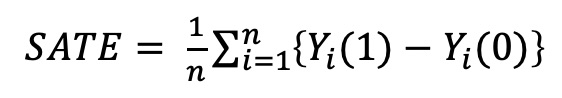
\includegraphics[width=0.7\linewidth]{SATE1}

\begin{itemize}
\tightlist
\item
  Essais contrôlés randomisés comme \textbf{norme d'excellence}
  (\emph{Gold standard})
\end{itemize}

\end{frame}

\begin{frame}{Essais contrôlés randomisés}
\protect\hypertarget{essais-controles-randomises-1}{}

\begin{itemize}
\tightlist
\item
  La SATE n'est pas directement observable.
\item
  Pour le groupe de traitement qui a reçu le traitement, nous avons
  observé le résultat moyen sous le traitement, mais nous ne savons pas
  quel aurait été leur résultat moyen sans le traitement.
\item
  Le même problème existe pour le groupe témoin car ce groupe ne reçoit
  pas le traitement et, par conséquent, nous n'observons pas le résultat
  moyen qui se produirait dans les conditions de traitement.
\item
  Pour estimer le résultat contrefactuel moyen du traitement, nous
  pouvons utiliser le résultat moyen observé du groupe témoin.
\item
  De même, nous pouvons utiliser le résultat moyen observé du groupe de
  traitement comme une estimation du résultat contrefactuel moyen pour
  le groupe de contrôle.
\item
  La Sate peut être estimée en calculant la différence entre le résultat
  moyen entre les groupes de traitement et témoin
\item
  En clair, la grande question de la causalité n'est qu'une question de
  soustraction :)
\end{itemize}

\end{frame}

\begin{frame}{Essais contrôlés randomisés}
\protect\hypertarget{essais-controles-randomises-2}{}

Dans un essai contrôlé randomisé (ECR), chaque unité est assignée de
manière aléatoire au groupe de traitement ou au groupe de contrôle. La
randomisation de l'assignation de traitement garantit que la différence
moyenne de résultats entre les groupes de traitement et de contrôle peut
être attribuée uniquement au traitement, car les deux groupes sont en
moyenne identiques pour toutes les caractéristiques de prétraitement
(observées et non observées).

\end{frame}

\begin{frame}{Essais contrôlés randomisés}
\protect\hypertarget{essais-controles-randomises-3}{}

\begin{enumerate}
\tightlist
\item
  \textbf{Forces}\\
\end{enumerate}

\begin{itemize}
\tightlist
\item
  \textbf{Validité interne} - mesure dans laquelle les hypothèses de
  causalité sont satisfaites dans l'étude
\end{itemize}

\begin{enumerate}
\setcounter{enumi}{1}
\tightlist
\item
  \textbf{Limites}
\end{enumerate}

\begin{itemize}
\tightlist
\item
  \textbf{Validité externe} - mesure dans laquelle les conclusions
  peuvent être généralisées au-delà d'une étude particulière
\item
  Explication causale faible
\item
  Considérations éthiques
\item
  Possibilité de contamination
\end{itemize}

\end{frame}

\hypertarget{applications}{%
\section{Applications}\label{applications}}

\begin{frame}{Exemple 1 discrimination raciale sur le marché du travail}
\protect\hypertarget{exemple-1-discrimination-raciale-sur-le-marche-du-travail}{}

\begin{enumerate}
\tightlist
\item
  \textbf{Question de recherche}
\end{enumerate}

\begin{itemize}
\tightlist
\item
  La discrimination raciale existe-t-elle sur le marché du travail?
\item
  Ou bien les disparités raciales dans le taux de chômage
  devraient-elles être attribuées à d'autres facteurs tels que les
  écarts raciaux dans le niveau d'instruction?
\end{itemize}

\begin{enumerate}
\setcounter{enumi}{1}
\tightlist
\item
  \textbf{Expérimentation}
\end{enumerate}

\begin{itemize}
\tightlist
\item
  En réponse aux annonces dans les journaux, les chercheurs ont envoyé
  les CV de candidats fictifs à des employeurs potentiels.
\item
  Changé seulement le nom du demandeur d'emploi

  \begin{itemize}
  \tightlist
  \item
    Noms afro-américains
  \item
    Noms à consonance caucasienne
  \end{itemize}
\item
  Les autres informations sont inchangées
\end{itemize}

\begin{enumerate}
\setcounter{enumi}{2}
\tightlist
\item
  \textbf{Variable dépendante}
\end{enumerate}

\begin{itemize}
\tightlist
\item
  Taux de rappel
\end{itemize}

\end{frame}

\begin{frame}{Exemple 1 discrimination raciale sur le marché du travail}
\protect\hypertarget{exemple-1-discrimination-raciale-sur-le-marche-du-travail-1}{}

\begin{itemize}
\item
  \textbf{Unité d'analyse}: Individus
\item
  \textbf{Variable de traitement} (variable d'intérêt causal)
  \textbf{T}: Nom à consonance afro-américain
\item
  \textbf{Groupe de traitement} (unités traitées): Afro-américains
\item
  \textbf{Groupe de contrôle} (unités non traitées): Caucasiens
\item
  \textbf{Réponse} (variable de réponse) \textbf{Y}: si un rappel a été
  effectué

  \begin{itemize}
  \tightlist
  \item
    Que signifie \textbf{``T cause Y''}?
  \item
    Contrefactuels, \textbf{``Quoi si''} : Les Afro-Américains
    auraient-ils été rappelés s'ils n'avaient pas de noms
    afro-américains?
  \end{itemize}
\end{itemize}

\end{frame}

\begin{frame}[fragile]{Exemple 1 discrimination raciale sur le marché du
travail}
\protect\hypertarget{exemple-1-discrimination-raciale-sur-le-marche-du-travail-2}{}

\begin{itemize}
\item
  \textbf{Deux résultats possibles}: Y(1) et Y(0)
\item
  \textbf{Effet causal}: \texttt{Y(1)\ -\ Y(0)}
\item
  \textbf{Problème fondamental d'inférence causale}: un seul des deux
  résultats potentiels est observable
\end{itemize}

\end{frame}

\begin{frame}{Exemple 1 discrimination raciale sur le marché du travail}
\protect\hypertarget{exemple-1-discrimination-raciale-sur-le-marche-du-travail-3}{}

\begin{itemize}
\tightlist
\item
  Comment pouvons-nous comprendre les contrefactuels?

  \begin{itemize}
  \tightlist
  \item
    L'association n'est pas un lien de causalité
  \item
    Trouvez une unité similaire! ==\textgreater{} \textbf{Matching}
  \item
    Est-ce-que Jamal n'a été rappelé à cause de sa race?
  \item
    Trouver une personne blanche qui ressemble à Jamal
  \end{itemize}
\item
  Le problème: on ne peut pas correspondre sur tout
\item
  Facteurs de \textbf{confusion non observés}: variables associées au
  traitement et au résultat ==\textgreater{} \textbf{biais de sélection}
\end{itemize}

\end{frame}

\begin{frame}{Exemple 1 discrimination raciale sur le marché du travail}
\protect\hypertarget{exemple-1-discrimination-raciale-sur-le-marche-du-travail-4}{}

\begin{itemize}
\tightlist
\item
  La clé pour comprendre la causalité est de penser au contrefactuel.
  L'inférence causale est une comparaison entre le factuel (ce qui s'est
  réellement passé) et le contrefactuel (ce qui se serait passé si une
  condition était différente).
\end{itemize}

\begin{figure}
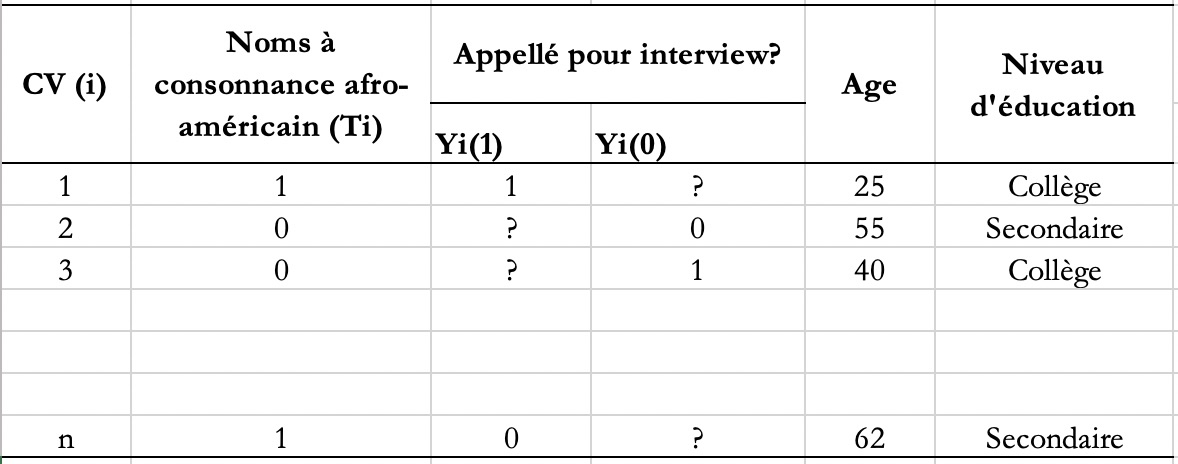
\includegraphics[width=1\linewidth]{factuel_contrafactuel} \caption{A caption}\label{fig:pressure}
\end{figure}

\begin{itemize}
\item
  La toute première observation des données de l'expérience de résumé
  montre qu'un employeur potentiel a reçu un CV avec un nom stéréotypé
  afro-américain et a décidé de rappeler.
\item
  Avec quoi remplaçons-nous les \textbf{?} dans le tableau?
\end{itemize}

\end{frame}

\begin{frame}[fragile]{Exemple 1 discrimination raciale sur le marché du
travail}
\protect\hypertarget{exemple-1-discrimination-raciale-sur-le-marche-du-travail-5}{}

\begin{verbatim}
##   firstname    sex  race call
## 1   Allison female white    0
## 2   Kristen female white    0
## 3   Lakisha female black    0
## 4   Latonya female black    0
## 5    Carrie female white    0
## 6       Jay   male white    0
\end{verbatim}

\end{frame}

\begin{frame}[fragile]{Exemple 1 discrimination raciale sur le marché du
travail}
\protect\hypertarget{exemple-1-discrimination-raciale-sur-le-marche-du-travail-6}{}

\begin{Shaded}
\begin{Highlighting}[]
\KeywordTok{freq}\NormalTok{(resume}\OperatorTok{$}\NormalTok{sex)}
\end{Highlighting}
\end{Shaded}

\begin{verbatim}
## Frequencies  
## resume$sex  
## Type: Character  
## 
##                Freq   % Valid   % Valid Cum.   % Total   % Total Cum.
## ------------ ------ --------- -------------- --------- --------------
##       female   3746     76.92          76.92     76.92          76.92
##         male   1124     23.08         100.00     23.08         100.00
##         <NA>      0                               0.00         100.00
##        Total   4870    100.00         100.00    100.00         100.00
\end{verbatim}

\end{frame}

\begin{frame}[fragile]{Exemple 1 discrimination raciale sur le marché du
travail}
\protect\hypertarget{exemple-1-discrimination-raciale-sur-le-marche-du-travail-7}{}

\begin{Shaded}
\begin{Highlighting}[]
\KeywordTok{freq}\NormalTok{(resume}\OperatorTok{$}\NormalTok{race)}
\end{Highlighting}
\end{Shaded}

\begin{verbatim}
## Frequencies  
## resume$race  
## Type: Character  
## 
##               Freq   % Valid   % Valid Cum.   % Total   % Total Cum.
## ----------- ------ --------- -------------- --------- --------------
##       black   2435     50.00          50.00     50.00          50.00
##       white   2435     50.00         100.00     50.00         100.00
##        <NA>      0                               0.00         100.00
##       Total   4870    100.00         100.00    100.00         100.00
\end{verbatim}

\end{frame}

\begin{frame}[fragile]{Exemple 1 discrimination raciale sur le marché du
travail}
\protect\hypertarget{exemple-1-discrimination-raciale-sur-le-marche-du-travail-8}{}

\begin{Shaded}
\begin{Highlighting}[]
\KeywordTok{freq}\NormalTok{(resume}\OperatorTok{$}\NormalTok{call)}
\end{Highlighting}
\end{Shaded}

\begin{verbatim}
## Frequencies  
## resume$call  
## 
##               Freq   % Valid   % Valid Cum.   % Total   % Total Cum.
## ----------- ------ --------- -------------- --------- --------------
##           0   4478     91.95          91.95     91.95          91.95
##           1    392      8.05         100.00      8.05         100.00
##        <NA>      0                               0.00         100.00
##       Total   4870    100.00         100.00    100.00         100.00
\end{verbatim}

\end{frame}

\begin{frame}[fragile]{Y'a-t-il discrimination ou pas?}
\protect\hypertarget{ya-t-il-discrimination-ou-pas}{}

\begin{Shaded}
\begin{Highlighting}[]
\KeywordTok{ctable}\NormalTok{(resume}\OperatorTok{$}\NormalTok{race, resume}\OperatorTok{$}\NormalTok{call)}
\end{Highlighting}
\end{Shaded}

\begin{verbatim}
## Cross-Tabulation, Row Proportions  
## race * call  
## Data Frame: resume  
## 
## ------- ------ -------------- ------------ ---------------
##           call              0            1           Total
##    race                                                   
##   black          2278 (93.6%)   157 (6.4%)   2435 (100.0%)
##   white          2200 (90.3%)   235 (9.7%)   2435 (100.0%)
##   Total          4478 (92.0%)   392 (8.0%)   4870 (100.0%)
## ------- ------ -------------- ------------ ---------------
\end{verbatim}

\begin{itemize}
\tightlist
\item
  SATE = 9,65 - 6,45 = 3,2\%
\end{itemize}

\end{frame}

\begin{frame}[fragile]{Est-ce que les deux groupes étaient similaires au
début?}
\protect\hypertarget{est-ce-que-les-deux-groupes-etaient-similaires-au-debut}{}

\begin{Shaded}
\begin{Highlighting}[]
\KeywordTok{ctable}\NormalTok{(resume}\OperatorTok{$}\NormalTok{race, resume}\OperatorTok{$}\NormalTok{sex)}
\end{Highlighting}
\end{Shaded}

\begin{verbatim}
## Cross-Tabulation, Row Proportions  
## race * sex  
## Data Frame: resume  
## 
## ------- ----- -------------- -------------- ---------------
##           sex         female           male           Total
##    race                                                    
##   black         1886 (77.5%)    549 (22.5%)   2435 (100.0%)
##   white         1860 (76.4%)    575 (23.6%)   2435 (100.0%)
##   Total         3746 (76.9%)   1124 (23.1%)   4870 (100.0%)
## ------- ----- -------------- -------------- ---------------
\end{verbatim}

\end{frame}

\hypertarget{exercices-de-groupes}{%
\section{Exercices de groupes}\label{exercices-de-groupes}}

\hypertarget{causalite-a-partir-des-donnees-observationnelles}{%
\section{Causalité à partir des données
observationnelles}\label{causalite-a-partir-des-donnees-observationnelles}}

\begin{frame}{Données observationnelles}
\protect\hypertarget{donnees-observationnelles}{}

\begin{itemize}
\item
  Souvent, nous ne pouvons pas randomiser le traitement pour des raisons
  éthiques et logistiques:
\item
  par exemple, tabagisme et cancer du poumon
\item
  Études observationnelles: traitement naturellement attribué
\item
  Plans d'observation passifs ou plans corrélationnels
\item
  Pas d'assignation aléatoire, pas de groupe de contrôle\ldots{}
\end{itemize}

\end{frame}

\begin{frame}{Données observationnelles}
\protect\hypertarget{donnees-observationnelles-1}{}

\begin{itemize}
\tightlist
\item
  Meilleure validité externe pour la généralisation au-delà de
  l'expérience
\item
  Validité interne plus faible:

  \begin{itemize}
  \tightlist
  \item
    les variables pré-traitement peuvent différer entre les groupes
    (traitement et contrôle)
  \end{itemize}

  \begin{enumerate}
  \item
    \textbf{biais de confusion (Confounding bias)} dû à ces différences
    : Une variable de prétraitement associée aux variables de traitement
    et de résultat s'appelle un facteur de confusion et constitue une
    source de biais de confusion dans l'estimation de l'effet du
    traitement.
  \item
    \textbf{biais de confusion non observée (Unobserved confounding)}
    constitue la ménace la plus importante car il est inobservé.
  \end{enumerate}
\end{itemize}

\end{frame}

\begin{frame}{Données observationnelles}
\protect\hypertarget{donnees-observationnelles-2}{}

\begin{enumerate}
\setcounter{enumi}{2}
\tightlist
\item
  \textbf{biais de sélection (selection bias)} de l'auto-sélection au
  traitement: Le biais de confusion dû à l'auto-sélection dans le groupe
  de traitement s'appelle un biais de sélection. Un biais de sélection
  apparaît souvent dans les études d'observation car les chercheurs
  n'ont aucun contrôle sur le destinataire du traitement.
\end{enumerate}

\begin{itemize}
\tightlist
\item
  Contrôle statistique devient alors nécessaire
\end{itemize}

\end{frame}

\begin{frame}{Données observationnelles}
\protect\hypertarget{donnees-observationnelles-3}{}

\begin{figure}
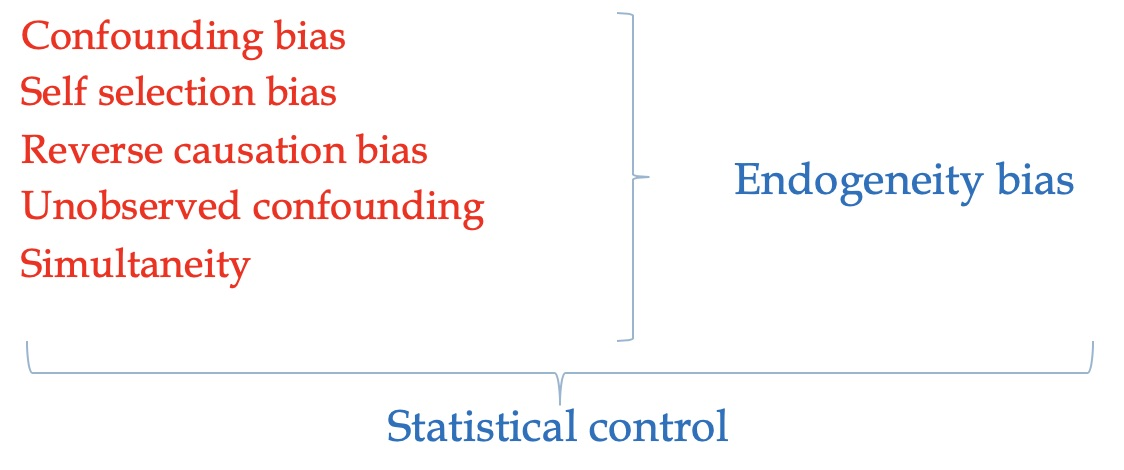
\includegraphics[width=1\linewidth]{endogeneite} \end{figure}

\end{frame}

\begin{frame}{Exemples}
\protect\hypertarget{exemples}{}

Il ya beaucoup d'accidents pendant les périodes de fête de Noël, donc la
fête de Noël cause des accidents.

\begin{figure}
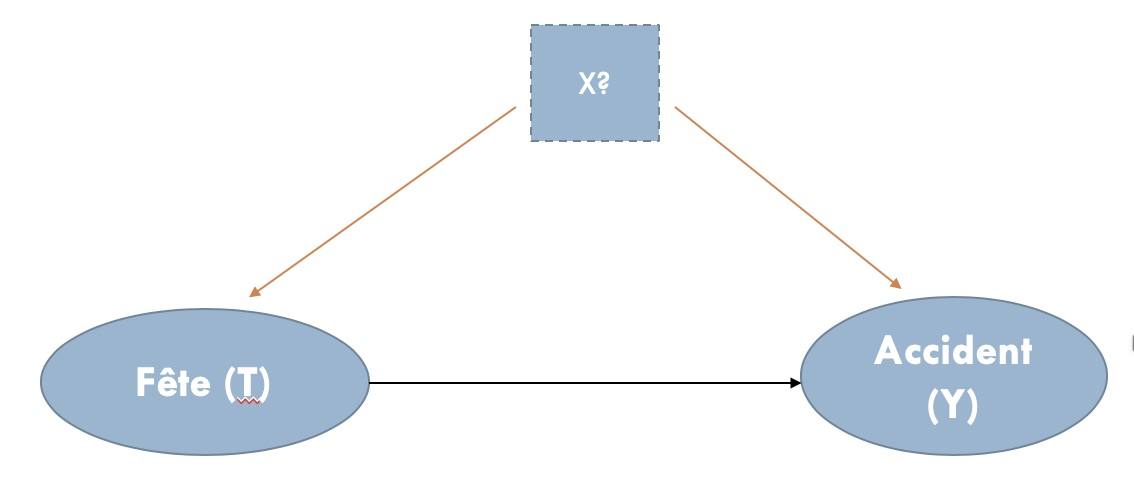
\includegraphics[width=0.8\linewidth]{confounding} \end{figure}

Problèmes?

\end{frame}

\begin{frame}{Exemples}
\protect\hypertarget{exemples-1}{}

\begin{itemize}
\tightlist
\item
  Adjiwanou, V. et LeGrand, T. (2013). Does antenatal care matter in the
  use of skilled birth attendance in rural Africa: A multi-country
  analysis, Social Science \& Medicine 86: 26-34.

  \begin{itemize}
  \tightlist
  \item
    Est-ce que le fait d'avoir des consultations prénatales entraîne un
    accouchement à l'hopital?
  \end{itemize}
\item
  Adjiwanou, V. (En revision). Stepfamilies in sub-Saharan Africa and
  their consequences in terms of children's well-being, Presented at the
  Population Association of America (PAA) 2017.

  \begin{itemize}
  \tightlist
  \item
    Est-ce que le fait de vivre avec son beau-père réduit les chances de
    scolarisation?
  \end{itemize}
\end{itemize}

\end{frame}

\hypertarget{solutions}{%
\section{Solutions}\label{solutions}}

\begin{frame}{Solution 1}
\protect\hypertarget{solution-1}{}

\begin{enumerate}
\tightlist
\item
  Comparaison transversale (Cross-section comparison)

  \begin{itemize}
  \tightlist
  \item
    Comparez les unités traitées avec les unités de contrôle après le
    traitement
  \item
    Hypothèse: les unités traitées et les unités de contrôle sont
    comparables
  \item
    Possibilité de confusion
  \end{itemize}
\end{enumerate}

\begin{figure}
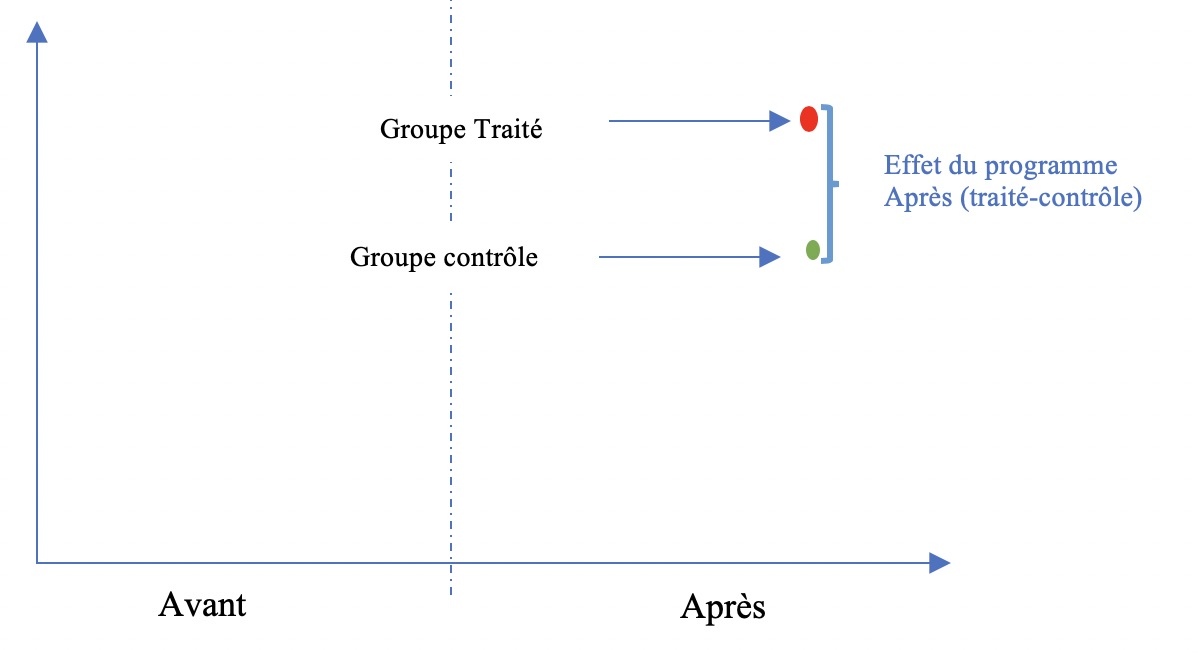
\includegraphics[width=0.8\linewidth]{cross_sectional} \end{figure}

\end{frame}

\begin{frame}{Solution 2}
\protect\hypertarget{solution-2}{}

\begin{enumerate}
\setcounter{enumi}{1}
\tightlist
\item
  Comparaison avant-après (Before\_and\_after comparison)

  \begin{itemize}
  \tightlist
  \item
    Comparez les mêmes unités avant et après le traitement
  \item
    Hypothèse: pas de variable de confusion qui change dans le temps
  \end{itemize}
\end{enumerate}

\begin{figure}
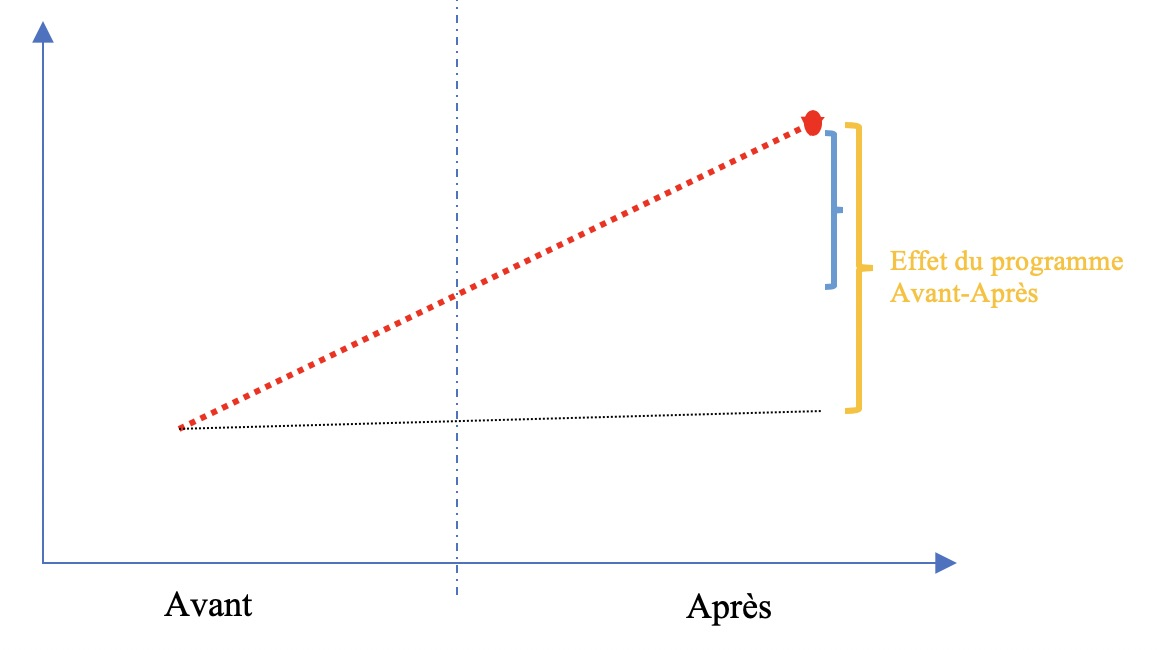
\includegraphics[width=0.8\linewidth]{Before-After} \end{figure}

\end{frame}

\begin{frame}{Solution 3}
\protect\hypertarget{solution-3}{}

\begin{enumerate}
\setcounter{enumi}{2}
\tightlist
\item
  Double différence (DD) - Difference-in-differences

  \begin{itemize}
  \tightlist
  \item
    Compare les individus entre périodes et entre traitement et contrôle
  \item
    Hypothèse: tendance temporelle parallèle
  \item
    Tient compte à la fois des facteurs de confusion spécifiques aux
    unités et variables dans le temps.
  \end{itemize}
\end{enumerate}

\begin{figure}
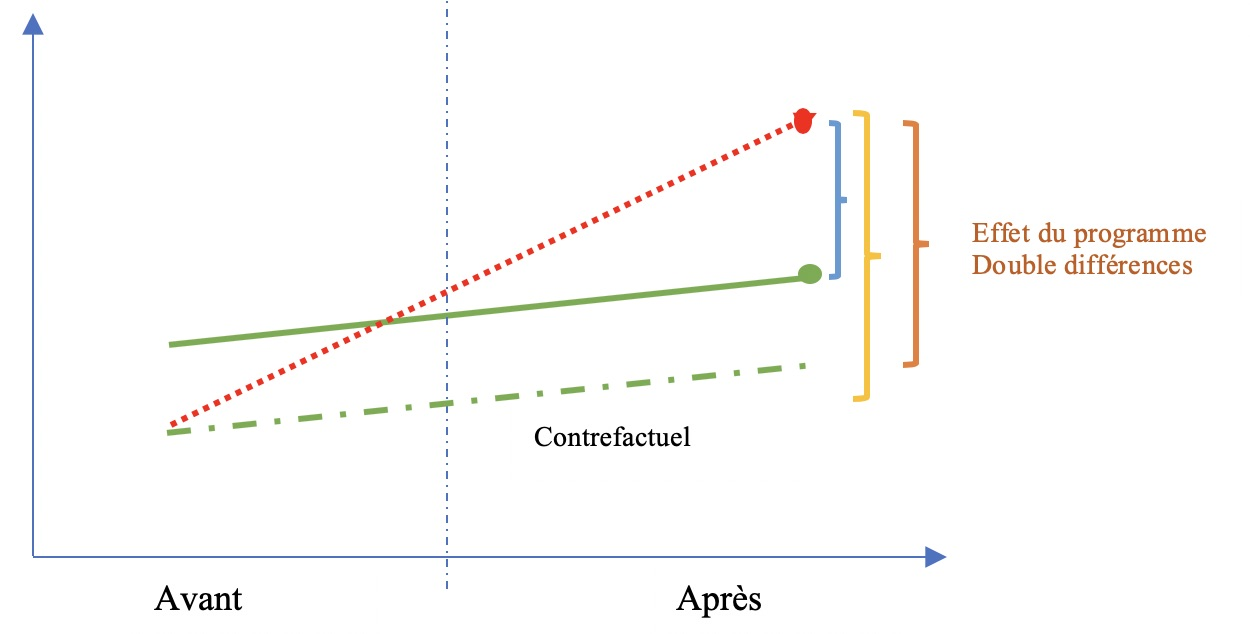
\includegraphics[width=0.8\linewidth]{Double_difference} \end{figure}

\end{frame}

\hypertarget{exercices-de-groupes-1}{%
\section{Exercices de groupes}\label{exercices-de-groupes-1}}

\begin{frame}{Comment l'augmentation du salaire minimum affecte-t-elle
l'emploi?}
\protect\hypertarget{comment-laugmentation-du-salaire-minimum-affecte-t-elle-lemploi}{}

\begin{itemize}
\tightlist
\item
  Débat actuel: augmentation du salaire minimum fédéral
\item
  De nombreux économistes estiment que cet effet sera négatif:

  \begin{itemize}
  \tightlist
  \item
    surtout pour les pauvres
  \item
    aussi pour toute l'économie
  \end{itemize}
\item
  Difficile de randomiser l'augmentation du salaire minimum
\item
  Deux chercheurs en sciences sociales ont testé cette technique en
  utilisant des chaînes de restauration rapide au New-Jersey (NJ) et en
  Pennsylvanie (PA).

  \begin{itemize}
  \tightlist
  \item
    En 1992, le salaire minimum dans le New Jersey a augmenté de 4,25
    dollars à 5,05 dollars
  \item
    En Pennsylvanie, il est demeuré à 4,25 \$
  \end{itemize}
\item
  NJ et PA (est) sont similaires
\item
  Les chaînes de restauration rapide au NJ et en PA sont similaires:
  prix, salaires, produits, etc.
\item
  Quel est l'impact de l'augmentation du salaire minimum au NJ?
\end{itemize}

\end{frame}

\begin{frame}{Données}
\protect\hypertarget{donnees}{}

\begin{figure}
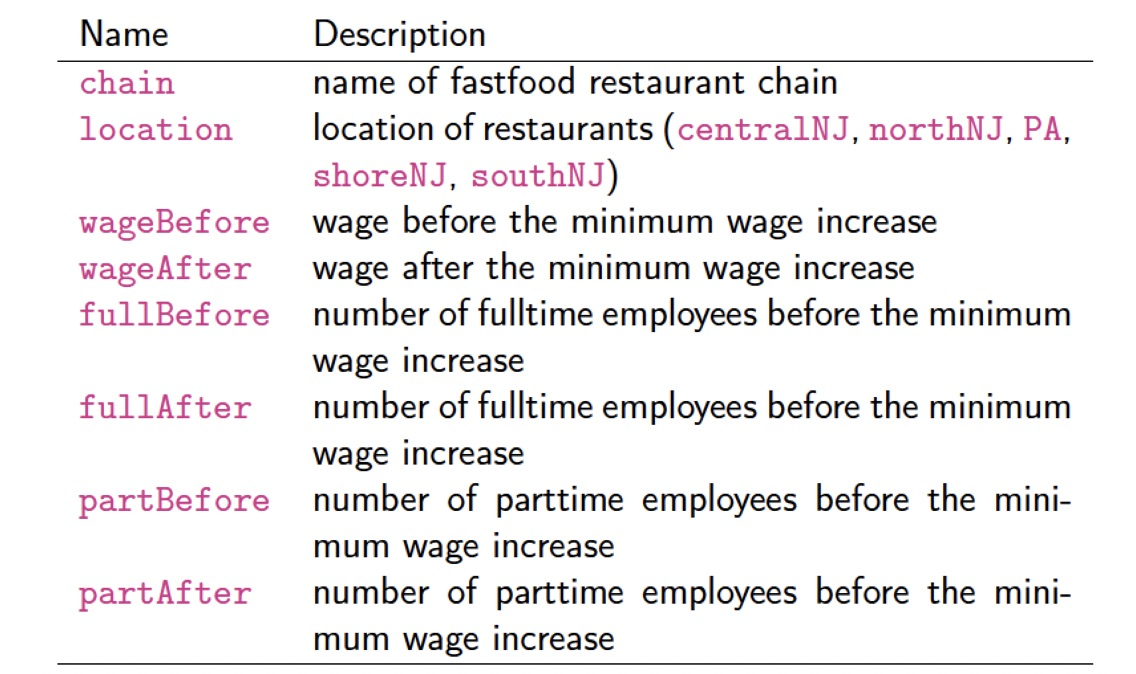
\includegraphics[width=0.8\linewidth]{minimum-wage} \end{figure}

\end{frame}

\begin{frame}[fragile]{Données}
\protect\hypertarget{donnees-1}{}

\begin{verbatim}
##        chain location wageBefore wageAfter fullBefore fullAfter partBefore
## 1     wendys       PA       5.00      5.25         20         0         20
## 2     wendys       PA       5.50      4.75          6        28         26
## 3 burgerking       PA       5.00      4.75         50        15         35
## 4 burgerking       PA       5.00      5.00         10        26         17
## 5        kfc       PA       5.25      5.00          2         3          8
## 6        kfc       PA       5.00      5.00          2         2         10
##   partAfter
## 1        36
## 2         3
## 3        18
## 4         9
## 5        12
## 6         9
\end{verbatim}

\end{frame}

\begin{frame}[fragile]{Réponse}
\protect\hypertarget{reponse}{}

\begin{itemize}
\tightlist
\item
  Variable dépendante: proportion de la main-d'oeuvre à temps plein.
\item
  Comparaison transversale
\end{itemize}

\begin{verbatim}
## # A tibble: 2 x 2
##   state fullPropAfter
##   <chr>         <dbl>
## 1 NJ            0.320
## 2 PA            0.272
\end{verbatim}

\end{frame}

\begin{frame}[fragile]{réponse}
\protect\hypertarget{reponse-1}{}

\begin{itemize}
\tightlist
\item
  Avant et après
\end{itemize}

\begin{verbatim}
##   PropBefore PropAfter diff_bef_aft_NJ
## 1  0.2965262  0.320401      0.02387474
\end{verbatim}

\end{frame}

\begin{frame}[fragile]{réponse}
\protect\hypertarget{reponse-2}{}

\begin{itemize}
\tightlist
\item
  Double différences
\end{itemize}

\begin{verbatim}
## # A tibble: 1 x 3
##       NJ      PA diff_in_diff
##    <dbl>   <dbl>        <dbl>
## 1 0.0239 -0.0377       0.0616
\end{verbatim}

\end{frame}

\hypertarget{pour-la-suite}{%
\section{Pour la suite}\label{pour-la-suite}}

\begin{frame}{Pour la suite}
\protect\hypertarget{pour-la-suite-1}{}

\begin{itemize}
\item
  R possède le meilleur package de graphique appellé ggplot
\item
  \url{https://www.datacamp.com/courses/data-visualization-with-ggplot2-1}
\item
  Vos travaux m'intéressent!
\end{itemize}

\end{frame}

\end{document}
